\chapter{Experiments}
\section{T-F Masking Estimations}
\subsection{IRM}

\subsection{cIRM}

\begin{figure}[H]
    \centering
    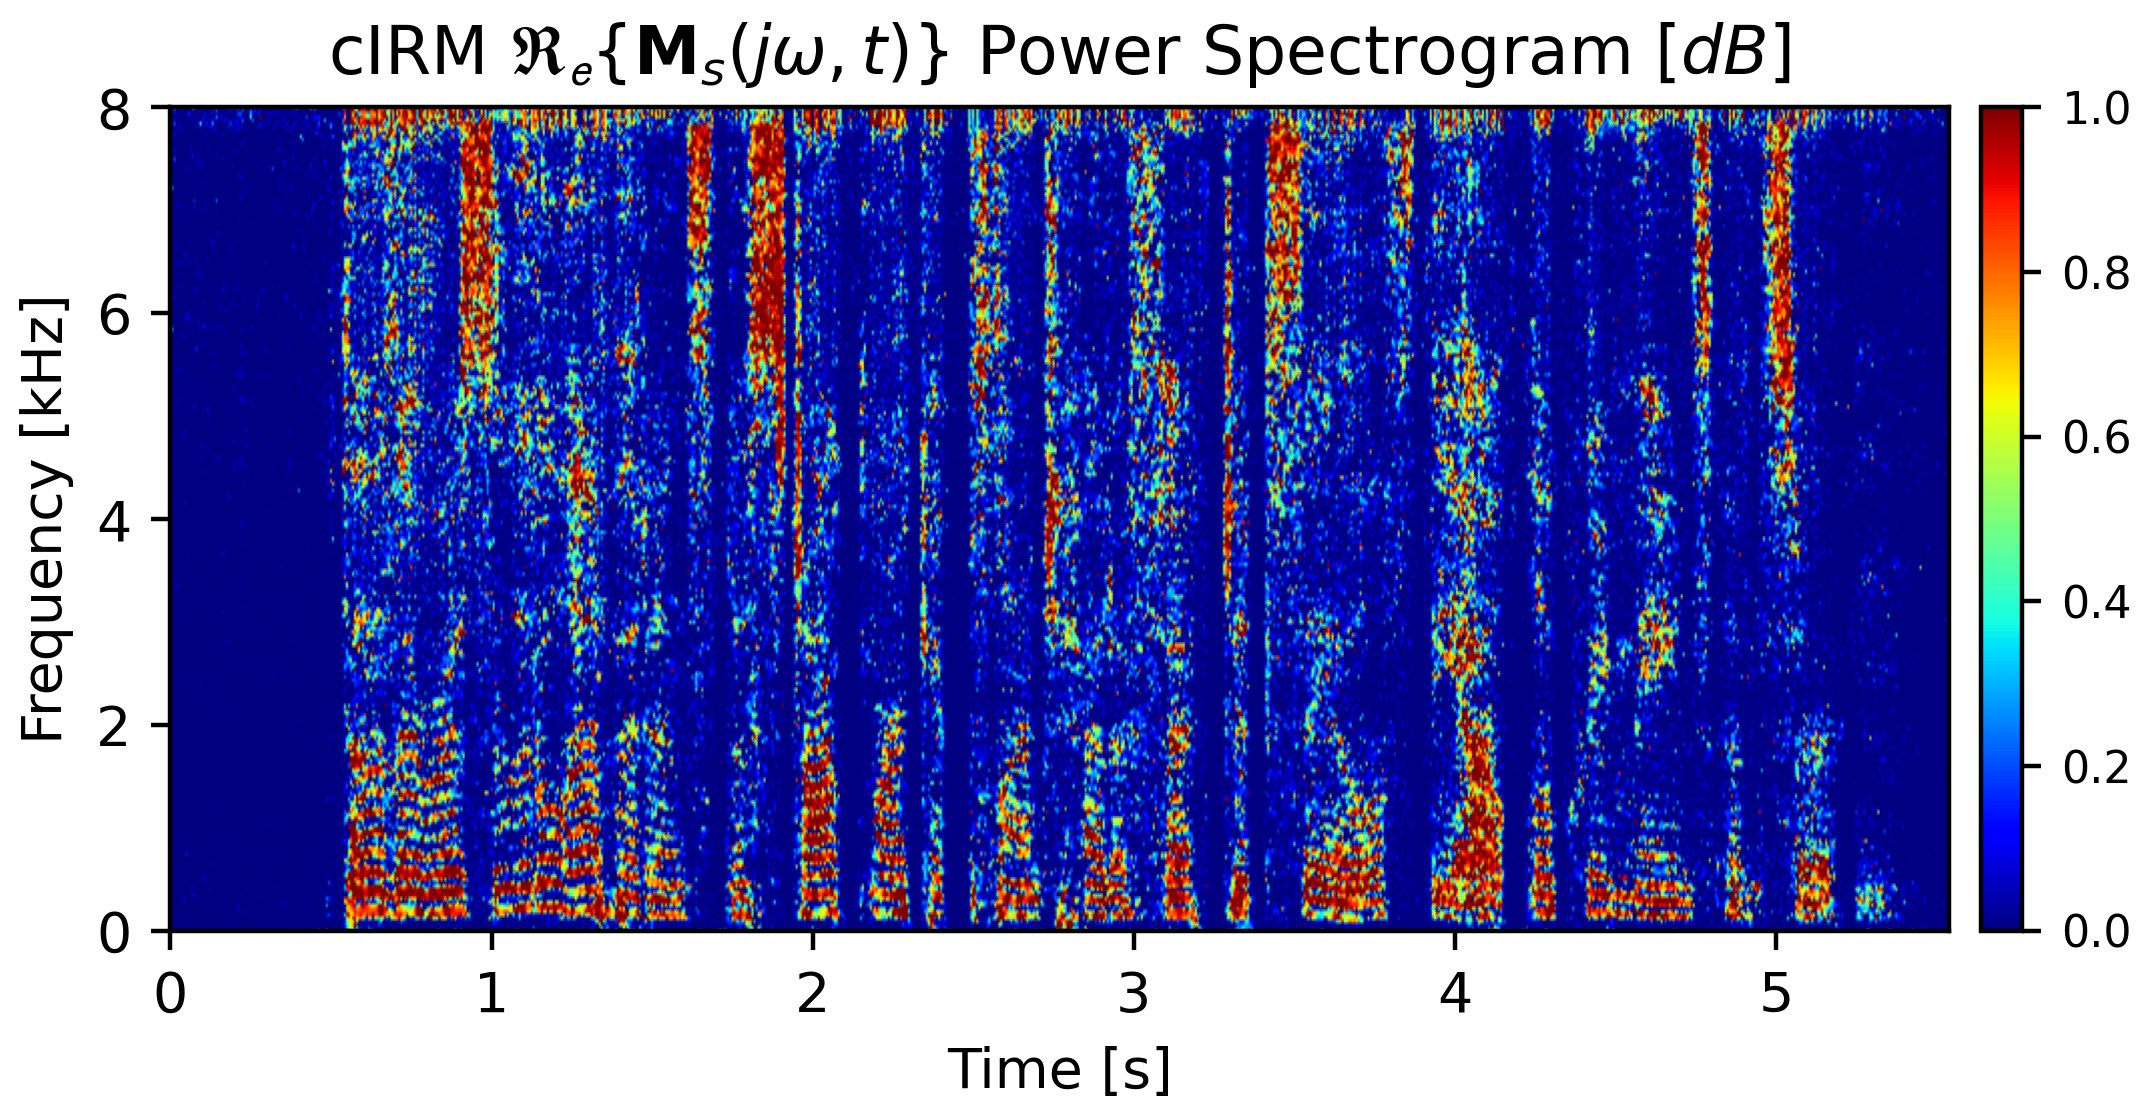
\includegraphics[width=0.75\linewidth]{Features/images/cIRM_real_mask}
    \caption{cIRM real mask}\label{fig:asr_5}
\end{figure}

\begin{figure}[H]
    \centering
    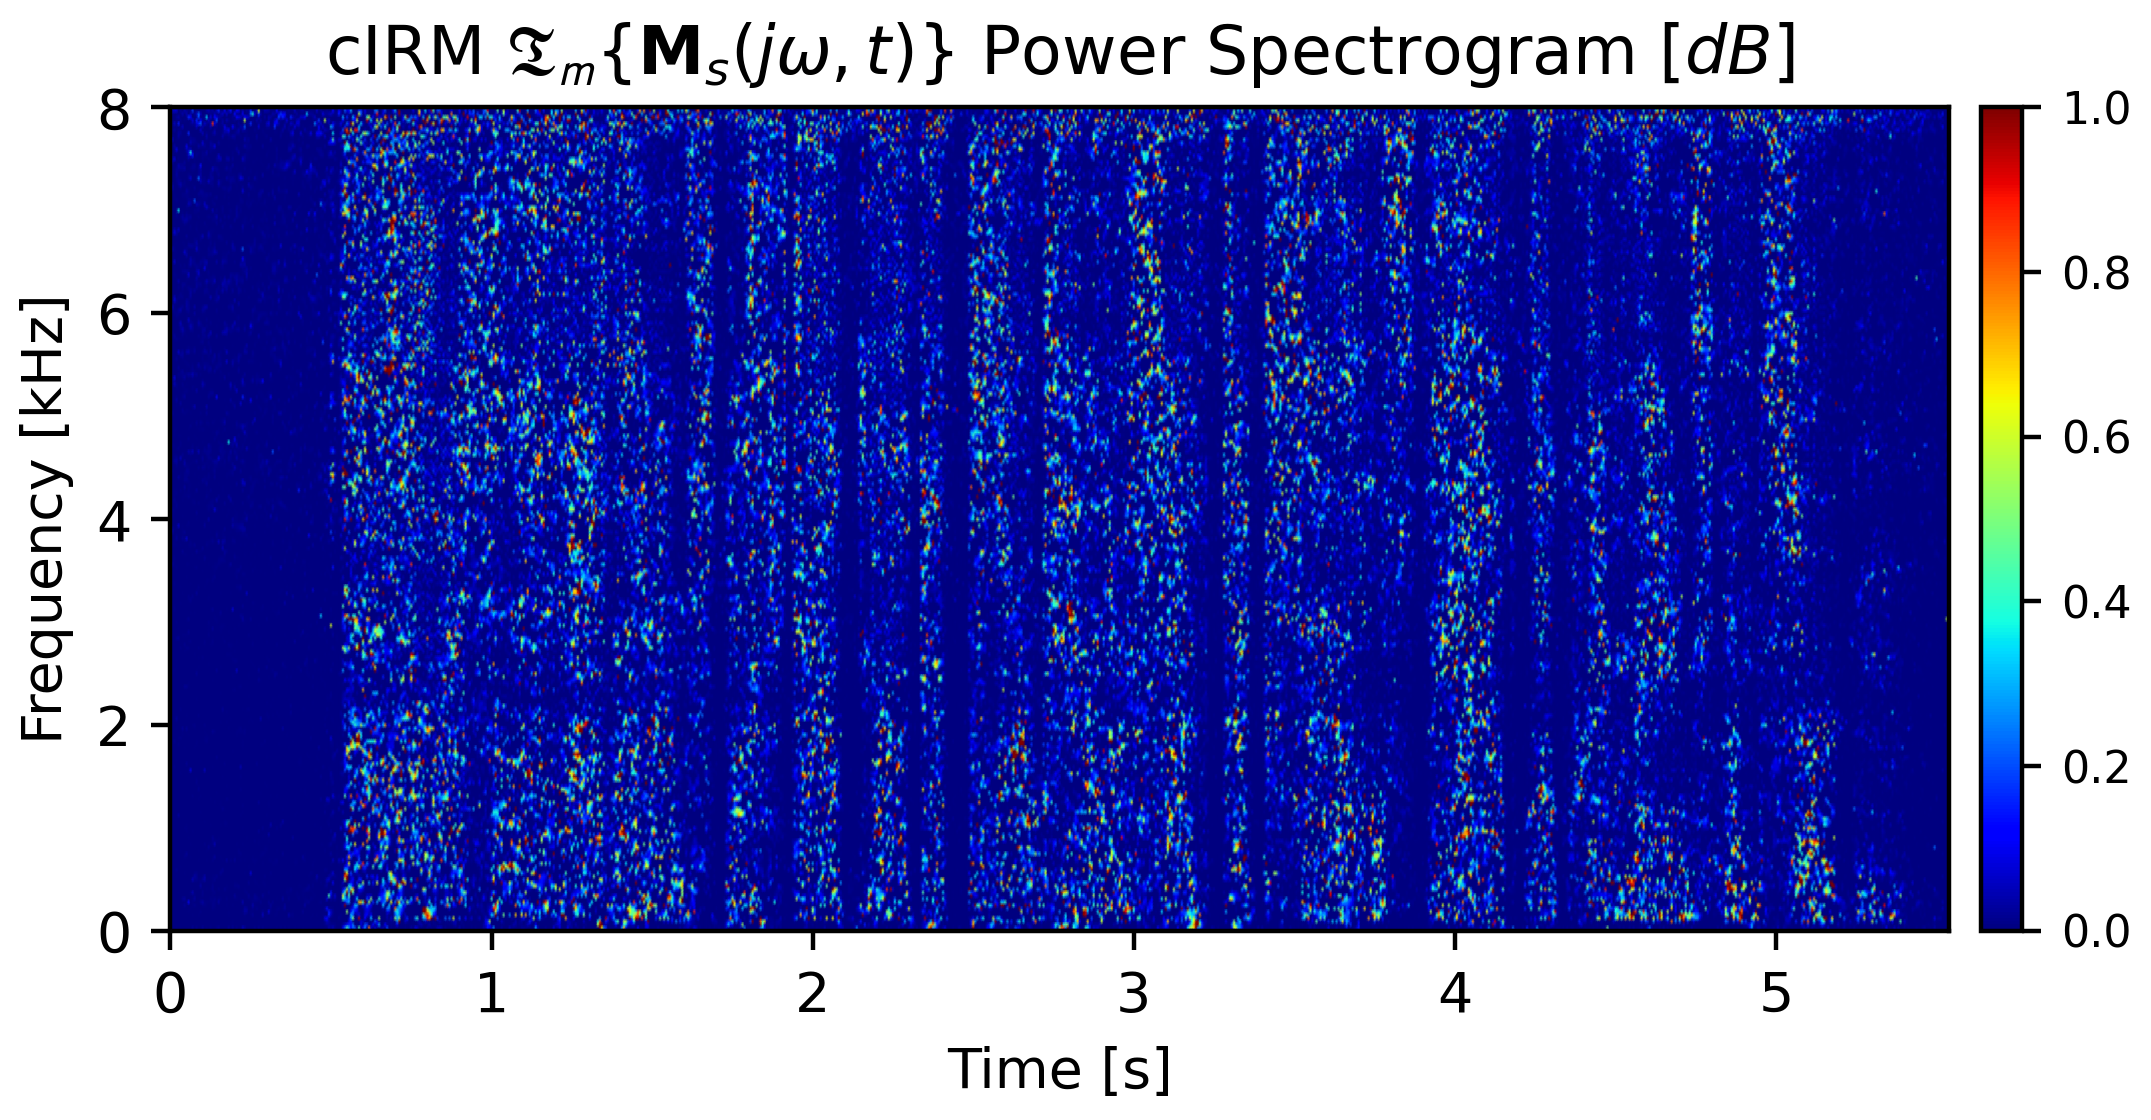
\includegraphics[width=0.75\linewidth]{Features/images/cIRM_imag_mask}
    \caption{cIRM imag mask}\label{fig:asr_5}
\end{figure}

\subsection{PSM}
\begin{figure}[H]
    \centering
    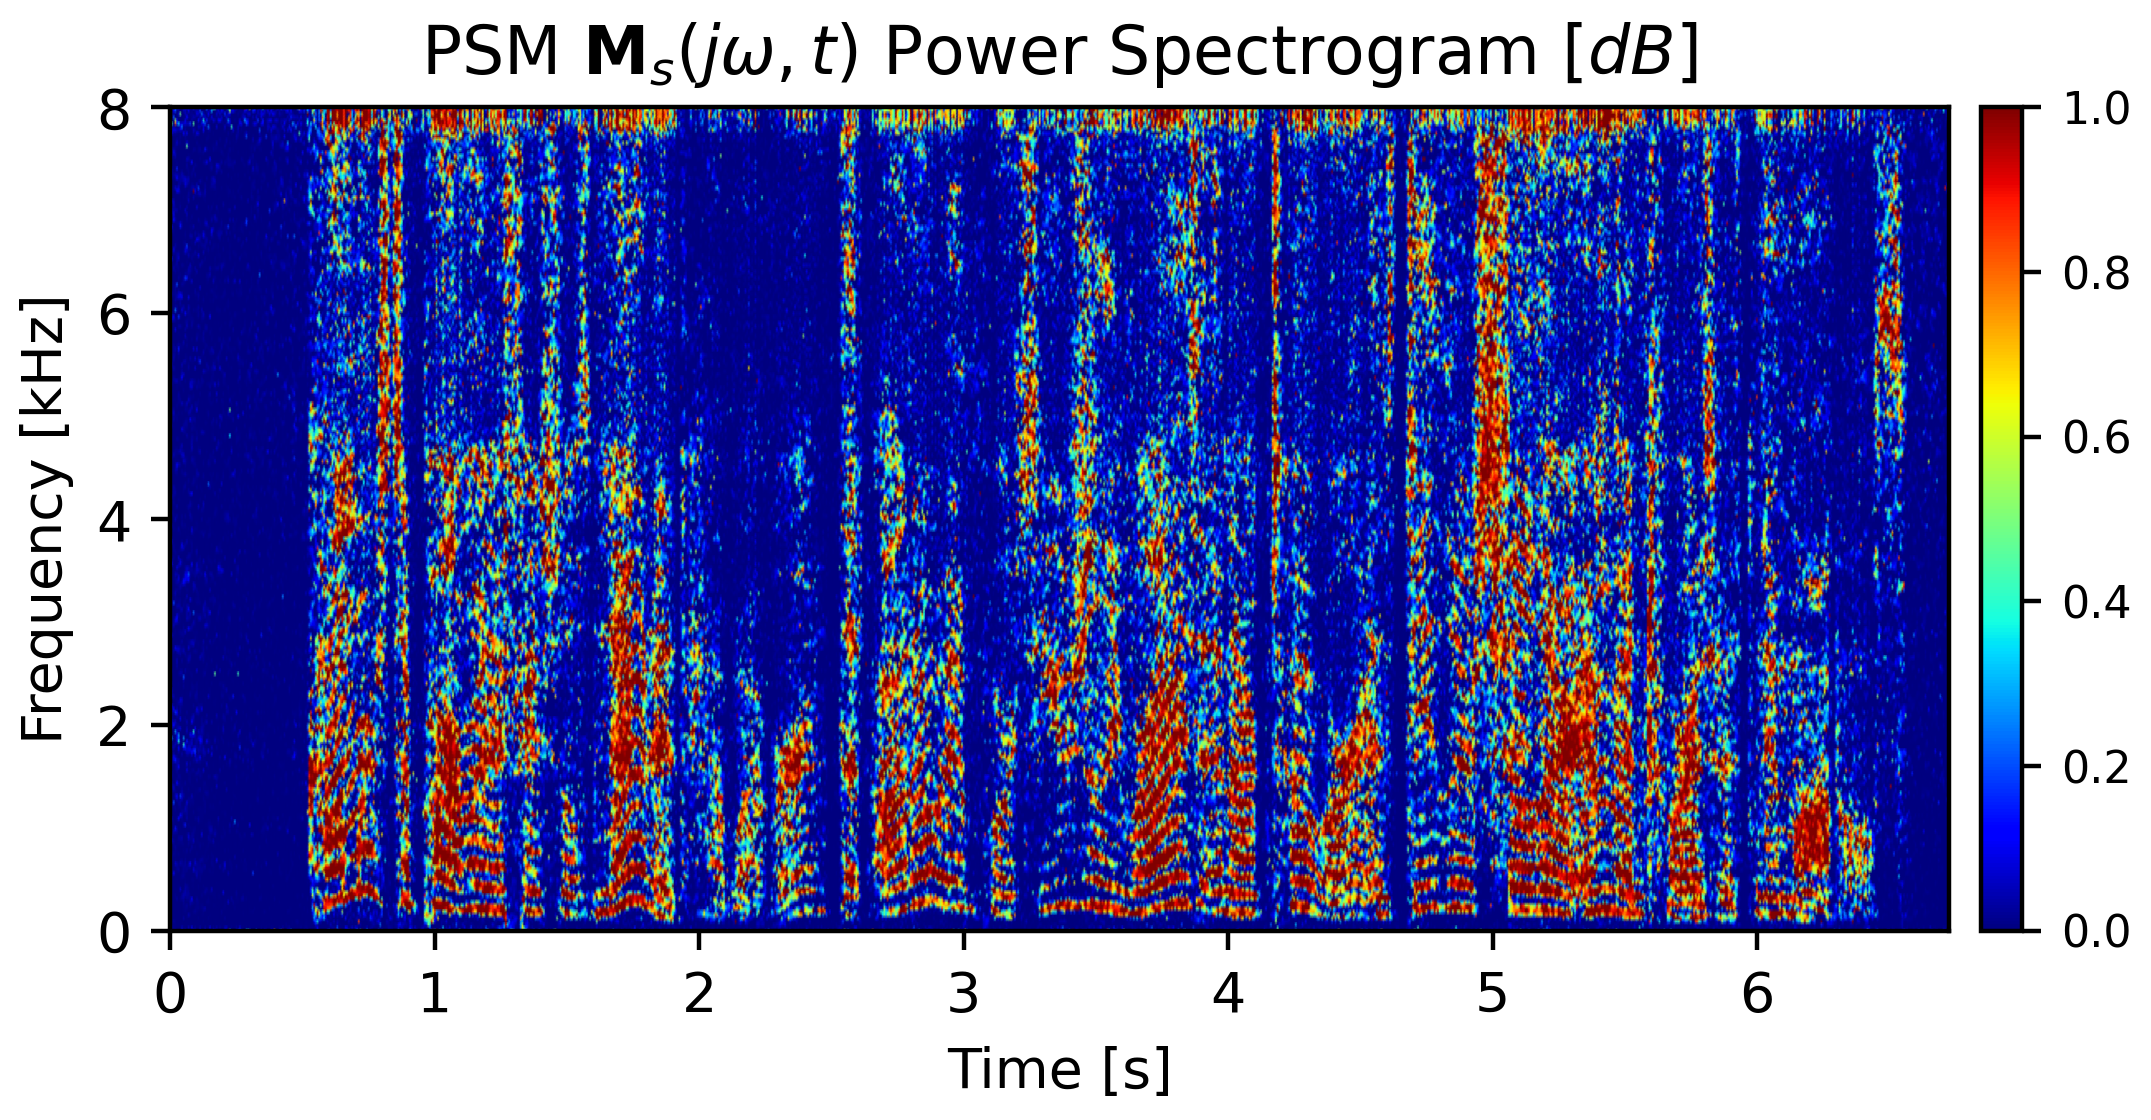
\includegraphics[width=0.75\linewidth]{Features/images/psm_mask}
    \caption{psm mask}\label{fig:asr_5}
\end{figure}

\subsection{ORM}
\begin{figure}[H]
    \centering
    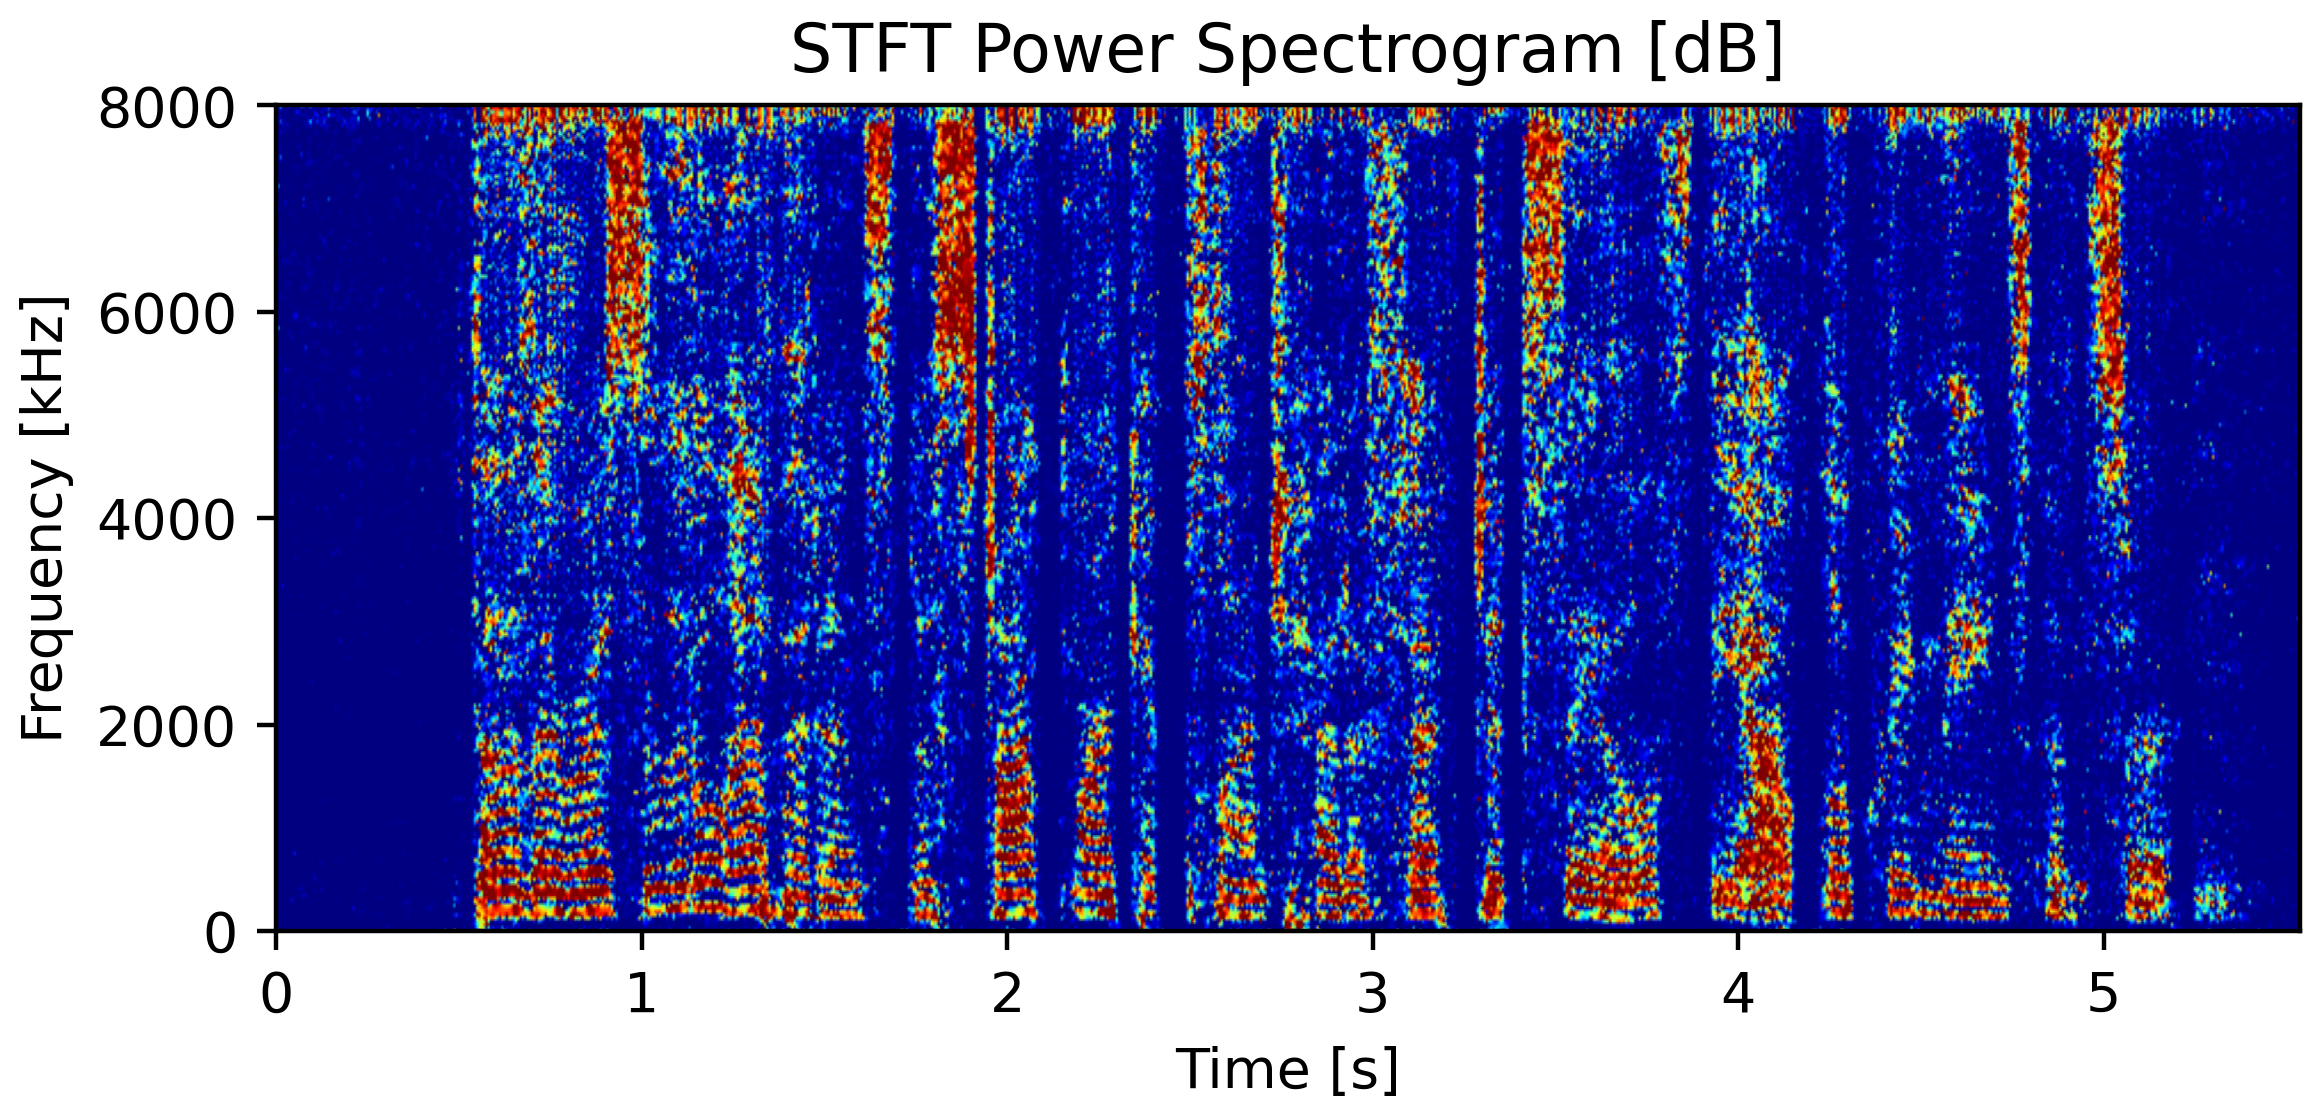
\includegraphics[width=0.75\linewidth]{Features/images/orm_mask}
    \caption{orm mask}\label{fig:asr_5}
\end{figure}


\begin{table}[H]
    % for more info see: https://www.overleaf.com/learn/latex/tables
    \centering
    % \hspace*{-2.8cm}
    \arrayrulecolor{mtblborder}
\begin{tabular}{ !{\color{mtblborder}\vrule}c!{\color{mtblborder}\vrule}cc|||cc| } 
    \hline

    \hline
    \rowcolor{mtblcaption}
    & \multicolumn{2}{c}{\color{white}\bf{Learnable Parameters} [Mil]}
    & \multicolumn{2}{c}{\color{white}\bf{Quant. (S16.11) Mem } [Mb]}\\         
    % \cline{2-8}
    
    \multirow{-2}{*}{\cellcolor{mtblcaption}\color{white}\bf{Targets} }
    & \cellcolor{mtbl} \color{black}{W/o (\(\Delta\),\(\Delta\Delta\))} 
    & \cellcolor{mtbl} \color{black}{W/ (\(\Delta\),\(\Delta\Delta\))}
    & \cellcolor{mtbl} \color{black}{W/o (\(\Delta\),\(\Delta\Delta\))} 
    & \cellcolor{mtbl} \color{black}{W (\(\Delta\),\(\Delta\Delta\))} \\
    % & \color{white}\bf{ORM} 
    % & \color{white}\bf{Clean} \\
    \hline

    \hline
    \rowcolor{mtblA} IRM  
        & 2.44 
        & 4.67
        & 39.0
        & 74.8 \\
    \hline
    
    \hline
    \rowcolor{mtbl} cIRM  
        & 3.76
        & 5.99
        & 60.1
        & 95.9 \\
    \hline

    \hline
    \rowcolor{mtblA} PSM  
        & 3.49
        & 5.73
        & 55.9
        & 91.7 \\
    \hline

    \hline
    \rowcolor{mtbl} ORM  
        & 3.50
        & 5.74
        & 56.0
        & 91.8 \\
    \hline
    
    \hline
\end{tabular}
\arrayrulecolor{black}
\caption{T-F Masks models learnable parameters vs. Required memory size}
\label{tbl:masks_l_params}
\end{table}


\section{Front-End Beamformers}
\subsection{IRM Beamformer}
\begin{figure}[H]
    \centering
    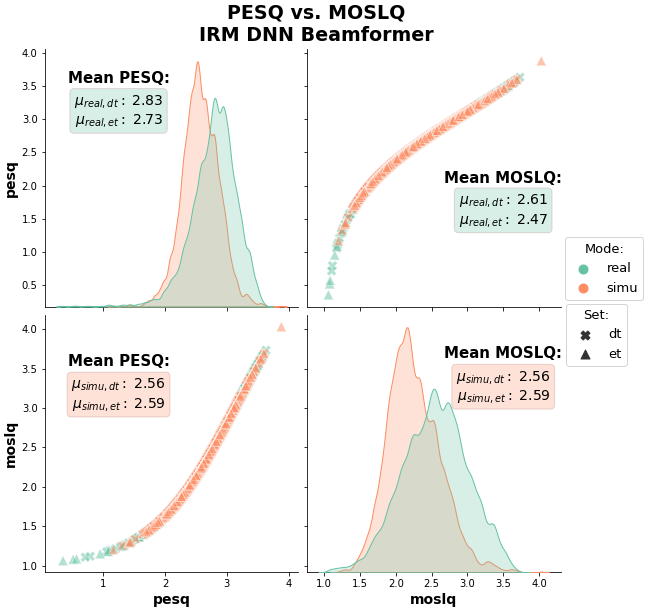
\includegraphics[width=\linewidth]{Experiments/images/irm_pesq_mosq}
    \caption{IRM beamformer PESQ vs. MOSLQ}\label{fig:irm_pesq_mosq}
\end{figure}

\begin{table}[H]
    % for more info see: https://www.overleaf.com/learn/latex/tables
    \centering
    \begin{tabular}{lr}
      \midrule
      Set & Utterances [\(N\)] \\
      \midrule
        Training    & 759,546   \\
        Dev/Valid   & 16,264   \\
        Test        & 16,236  \\
       \bottomrule
    \end{tabular}
    \caption{IRM beamformer PESQ \& MOSLQ}\label{tbl:comvoice_set_dstrb}
\end{table}

\subsection{cIRM Beamformer}
\begin{figure}[H]
    \centering
    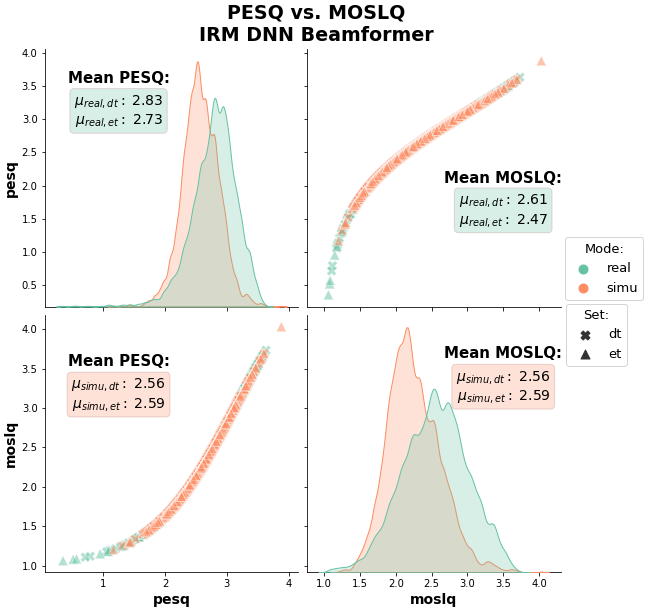
\includegraphics[width=\linewidth]{Experiments/images/irm_pesq_mosq}
    \caption{IRM beamformer PESQ vs. MOSLQ}\label{fig:cirm_pesq_mosq}
\end{figure}

% \section{Engines}




% \subsection{FB Transformer}

% \subsection{MFCC Transformer}

% \subsection{RFCC Transformer}
% kldiv loss = seqloss
% ctc loss

% \begin{equation}
%     \ell = \omega_{_{ctc}}  \ell_{_{ctc}} + (1 - \omega_{_{ctc}}) \cdot \ell_{_{seq}}
% \end{equation}




% \chapter{Scaling methods}



% \begin{table}
%     \centering
%     \begin{tabular}
%         {!{\color[HTML]{00638a}\vrule}l
%         !{\color[HTML]{00638a}\vrule}l
%         llllll
%         !{\color[HTML]{00638a}\vrule}}
%         \arrayrulecolor[HTML]{00638a}\hline
%         \rowcolor[rgb]{0.6,0.757,0.945}  &                                    &                                    &                                    &                                    &                                    &                                    &                                     \\ 
%         \arrayrulecolor[HTML]{00638a}\cline{2-8}
%         \multirow{-2}{*}{{\cellcolor[rgb]{0.6,0.757,0.945}}}               &                                    &                                    &                                    &                                    &                                    &                                    &                                     \\ 
%         \arrayrulecolor[HTML]{00638a}\hline
%         \multirow{2}{*}{}                                                  & {\cellcolor[rgb]{0.6,0.757,0.945}} & {\cellcolor[rgb]{0.6,0.757,0.945}} & {\cellcolor[rgb]{0.6,0.757,0.945}} & {\cellcolor[rgb]{0.6,0.757,0.945}} & {\cellcolor[rgb]{0.6,0.757,0.945}} & {\cellcolor[rgb]{0.6,0.757,0.945}} & {\cellcolor[rgb]{0.6,0.757,0.945}}  \\ 
%         \arrayrulecolor[HTML]{00638a}\cline{2-8}
%                                                                        &     
%                                                                     &                                    &                                    &                                    &                                    &                                    &   \\ 
%         \arrayrulecolor[HTML]{00638a}\hline
%     \end{tabular}
%     \arrayrulecolor{black}
%     \end{table}


% \begin{table}[H]
%     % for more info see: https://www.overleaf.com/learn/latex/tables
%     \centering
%     \arrayrulecolor[HTML]{00638a}
% \begin{tabular}{ !{\color[HTML]{00638a}\vrule}c!{\color[HTML]{00638a}\vrule}ccccccc| } 
%     \hline

%     \hline
%     \rowcolor[HTML]{00a5ef} \color{white}\bf{Id} & \color{white}\bf{ASR Tr.} & \color{white}\bf{Noisy} & \color{white}\bf{IRM} & \color{white}\bf{cIRM} & \color{white}\bf{PSM} & \color{white}\bf{ORM} & \color{white}\bf{Clean} \\
%     \hline

%     \hline
%     \rowcolor[HTML]{ddf4ff}                         & 28.62/32.02 & 46.19 & 27.78 & - & - & - & 17.55 \\
%     \cline{2-8}
%     \multirow{-2}{*}{\cellcolor[HTML]{ddf4ff}\#1(5)}   & 14.03/17.78 & 27.06 & 13.73 & - & - & - & 7.72 \\ 
%     \hline

%     \hline
%     \rowcolor[HTML]{ddf4ff}\cellcolor[HTML]{ffffff} & 28.38/31.61 & - & - & - & - & - & - \\
%     \cline{2-8}
%     \multirow{-2}{*}{\#2(15)}                           & 13.27/16.68 & - & - & - & - & - & - \\ 
%     \hline
    
%     \hline
%     \rowcolor[HTML]{ddf4ff}                         & 28.09/31.18 & 46.25 & 28.03 & - & - & - & 18.46 \\
%     \cline{2-8}
%     \multirow{-2}{*}{\cellcolor[HTML]{ddf4ff}\#3(12)}   & 13.28/16.53 & 26.56 & 13.35 & - & - & - & 7.39 \\ 
%     \hline

%     \hline
%     \rowcolor[HTML]{ddf4ff}\cellcolor[HTML]{ffffff} & 28.77/31.6 & - & - & - & - & - & - \\
%     \cline{2-8}
%     \multirow{-2}{*}{\#4(22)}                           & 14.06/16.42 & - & - & - & - & - & - \\ 
%     \hline
    
%     \hline
%     \rowcolor[HTML]{ddf4ff}                         & 28.92/32.32 & - & - & - & - & - & - \\
%     \cline{2-8}
%     \multirow{-2}{*}{\cellcolor[HTML]{ddf4ff}\#5(23)}   & 13.53/17.05 & - & - & - & - & - & - \\ 
%     \hline

%     \hline
%     \rowcolor[HTML]{ddf4ff}\cellcolor[HTML]{ffffff} & 28.29/31.50 & - & - & - & - & - & - \\
%     \cline{2-8}
%     \multirow{-2}{*}{\#6(70)}                           & 13.42/16.72 & - & - & - & - & - & - \\ 
%     \hline
    
%     \hline
%     \rowcolor[HTML]{ddf4ff}                         & 28.26/31.51 & - & - & - & - & - & - \\
%     \cline{2-8}
%     \multirow{-2}{*}{\cellcolor[HTML]{ddf4ff}\#7(72)}   & 13.14/16.53 & - & - & - & - & - & - \\ 
%     \hline

%     \hline
%     \rowcolor[HTML]{ddf4ff}\cellcolor[HTML]{ffffff} & 29.60/35.00 & 45.79 & 28.07 & - & - & - & 19.23 \\
%     \cline{2-8}
%     \multirow{-2}{*}{\#8(100)}                           & 13.57/17.38 & 25.76 & 12.97 & - & - & - & 7.61 \\ 
%     \hline

%     \hline
%     \rowcolor[HTML]{ddf4ff}                         & 29.46/32.06 & 46.71 & 28.51 & - & - & - & 18.79 \\
%     \cline{2-8}
%     \multirow{-2}{*}{\cellcolor[HTML]{ddf4ff}\#9(13)}   & 14.16/17.77 & 26.59 & 14.03 & - & - & - & 7.84 \\ 
%     \hline

%     \hline
% \end{tabular}
% \arrayrulecolor{black}
% \caption{\bf{ IQRD Performance:} Latency and Resource Utilization vs Channel Count for XCZU3EG FPGA}
% \label{tbl:IQRD_perf}
% \end{table}
% \begin{table}[H]
%     % for more info see: https://www.overleaf.com/learn/latex/tables
%     \centering
%     \begin{tabular}{|c|r|r|r|r|r|}
%       \hline
%       Id & ASR Tr. & FF & LUT & DSP48 & BRAM \\
%       \hline
%       \multirow{2}3  & 4.80  &   3889 (27.6\%) &    3901 (54.9\%) &   90 (25.0\%) & 0 (0.0\%) \\
%       & 4.80  &   3889 (27.6\%) &    3901 (54.9\%) &   90 (25.0\%) & 0 (0.0\%) \\
%         4  & 6.34  &  63657 (45.1\%)                 &   64149 (90.4\%)                  &  144 (40.0\%) & 0 (0.0\%) \\
%         8  & 12.50 & 231199 (\textcolor{red}{164\%}) &  252446 (\textcolor{red}{356\%})  &  272 (75.6\%) & 0 (0.0\%) \\
%         16 & 24.82 & 895377 (\textcolor{red}{635\%}) & 1040992 (\textcolor{red}{1466\%}) &  144 (40.0\%) & 0 (0.0\%) \\
%        \hline
%     \end{tabular}
%     \caption{\bf{ IQRD Performance:} Latency and Resource Utilization vs Channel Count for XCZU3EG FPGA}
%     \label{tbl:IQRD_perf}
% \end{table}

